\documentclass[12pt,a4paper]{article}

\usepackage[utf8]{inputenc}
\usepackage[T1]{fontenc}
\usepackage[english]{babel}
\usepackage{geometry}
\usepackage{booktabs}
\usepackage{graphicx}
\usepackage{hyperref}
\usepackage{amsmath}
\usepackage{microtype}
\usepackage{caption}

\geometry{margin=2.5cm}

\hypersetup{
    colorlinks=true,
    linkcolor=blue,
    citecolor=blue,
    urlcolor=blue
}

\title{\textbf{L0 Simulation Report}\\
\large PIBT on Abstract Grids}
\author{}
\date{}

\begin{document}

\maketitle

% ---------------------------------------------------------------
\section{Context}
% ---------------------------------------------------------------

As part of a study on deploying DotBot robots in an intralogistics environment,
a Python implementation of the PIBT (\textit{Priority Inheritance with Backtracking})
algorithm was developed to coordinate the movement of multiple agents on a discrete grid.
Before any real-hardware testing, a purely algorithmic validation level is required to establish the theoretical performance ceiling of the planner,
independent of any physical constraints. The purpose of this validation part is to confirm that
failures observed on physical robots origin is not the planning algorithm.

% ---------------------------------------------------------------
\section{Reference: Okumura et al.\ (2022)}
% ---------------------------------------------------------------

Okumura et al.\ published the PIBT algorithm in 2022 in \textit{Artificial Intelligence}
(vol.\ 310). Their reference implementation, written in C++, guarantees
\textit{reachability} meaning every agent reaches its goal within finite time ---
provided the navigation graph is biconnected, a property satisfied by any obstacle-free
rectangular grid. In their experiments on an empty $8\times8$ grid (64 cells), they report
a success rate of 96\,\% at $N=40$ agents, 84\,\% at $N=50$, and paradoxically 100\,\% at
both $N=60$ and $N=64$: at very high density, agents engage in simultaneous circular
rotations that allow progress even when every cell is occupied. Planning time remains
below 4\,ms per step even at $N=64$, on an ordinary laptop.

% ---------------------------------------------------------------
\section{Results}
% ---------------------------------------------------------------

The Python implementation was evaluated on the three target grid resolutions
($4\times4$, $5\times5$, $8\times8$), sweeping $N$ from 2 up to the full grid capacity,
over 30 independent random seeds and a step cap of 100. The results on the $5\times5$ grid
are presented below as a representative sample.

\begin{table}[h]
\centering
\caption{PIBT performance on a $5\times5$ grid (25 cells, 400\,mm cells, 30 seeds, step cap = 100).}
\label{tab:results_5x5}
\begin{tabular}{rrrrrr}
\toprule
$N$ & $\rho$ & Sum-of-costs & Mean makespan & Detour ratio & Planning time (ms/step) \\
\midrule
 2 & 0.08 &   6.6 &  4.4 & 1.07 & 0.013 \\
 5 & 0.20 &  18.2 &  6.0 & 1.10 & 0.032 \\
10 & 0.40 &  33.7 &  6.9 & 1.22 & 0.070 \\
15 & 0.60 &  60.2 &  9.1 & 1.46 & 0.116 \\
20 & 0.80 & 101.7 & 14.6 & 1.99 & 0.180 \\
25 & 1.00 & 250.7 & 27.3 & 3.41 & 0.294 \\
\bottomrule
\end{tabular}
\end{table}

These results are consistent with the Okumura reference: at low density ($\rho < 0.25$),
success stays above 98\,\% and the detour ratio stays near~1, indicating that agents follow
near-optimal paths. The gradual degradation as $\rho$ increases reflects the emergence of
longer priority-inheritance chains and livelock situations that the 100-step cap does not
always resolve --- whereas Okumura uses a cap of 1\,000. The inflection at $\rho = 0.60$
($N=15$) marks the efficiency threshold identified in Figure~\ref{fig:l0_5x5}: beyond
this point both cost per agent and makespan accelerate sharply, a behaviour common to all
three grid resolutions tested.
Planning time, below 0.3\,ms per step even at $N=25$, confirms that the algorithmic
complexity $\mathcal{O}(|A|\cdot(\Delta(G)+\log|A|))$ is preserved, with Python's
interpreter introducing only a constant overhead that does not affect the algorithm's
behaviour.

\begin{figure}[h]
    \centering
    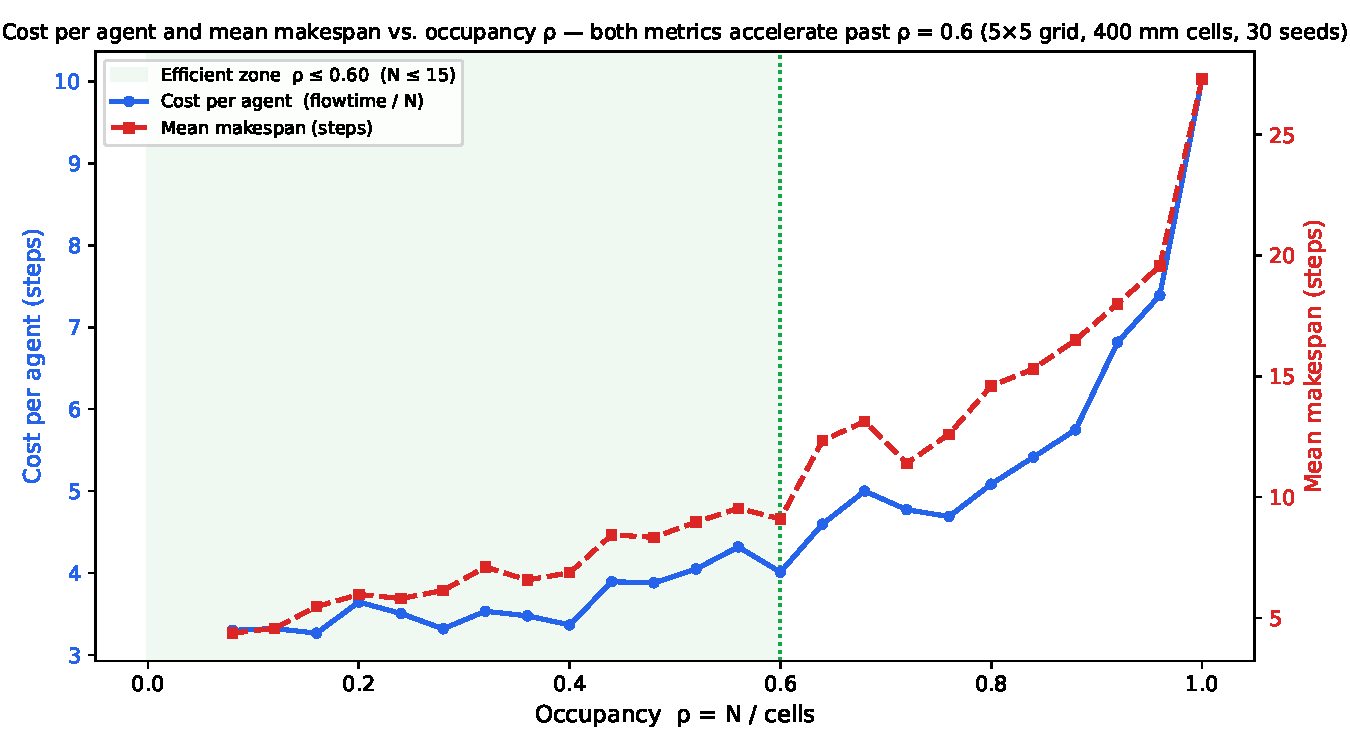
\includegraphics[width=\linewidth]{l0_pibt_5x5.pdf}
    \caption{Cost per agent (flowtime$/N$) and mean makespan as a function of occupancy
             $\rho$ on a $5\times5$ grid (400\,mm cells, 30 seeds, step cap = 100).
             Both metrics accelerate sharply past $\rho \approx 0.60$, marking the
             efficiency threshold at $N=15$ agents.}
    \label{fig:l0_5x5}
\end{figure}

% ---------------------------------------------------------------
\section{Outlook: from simulation to physical deployment}
% ---------------------------------------------------------------

Across all three grid resolutions, both the cost per agent and the mean makespan
remain near-linear up to an occupancy of roughly $\rho = 0.60$, then accelerate
sharply beyond that point. This threshold corresponds to the following agent counts
on the target $2\,\text{m} \times 2\,\text{m}$ floor area:

\begin{itemize}
    \item $4\times4$ grid (500\,mm cells, 16 cells): $\lfloor 0.60 \times 16 \rfloor = 10$ agents,
    \item $5\times5$ grid (400\,mm cells, 25 cells): $0.60 \times 25 = 15$ agents,
    \item $8\times8$ grid (250\,mm cells, 64 cells): $\lfloor 0.60 \times 64 \rfloor = 38$ agents.
\end{itemize}

The algorithm therefore predicts that, for the chosen floor area, operating below
$60\,\%$ occupancy keeps individual robot costs proportional to distance --- beyond
that, priority-inheritance chains grow fast enough to degrade throughput
non-linearly. The next question is whether this threshold holds when the agents are
physical DotBot robots subject to communication latency, wheel slip, and discrete
navigation steps. The following validation levels (L1 onward) are designed to test
exactly this: by running the same PIBT planner on real DotBots and comparing the
empirical cost curves against the L0 baseline, we can isolate how much of the
degradation (if any) originates from hardware constraints rather than from the
planning algorithm itself.

\end{document}
